%instiki:category: QuantumFieldTheory
\chapter{$S$--matrix}
\label{cha:s-matrix} %noinstiki
%instiki:
%instiki:***
%instiki:
%instiki:[[Beyond|Contents]]
%instiki:
%instiki:***
%instiki:
%instiki:* [Relativistic and no relativistic normalizations](#relat-no-relat)
%instiki:
%instiki:* [Decay Rates](#decay-rates)
%instiki:
%instiki:* [Cross Section](#cross-section)
%instiki:
%instiki:* [Backup](#backup)
%instiki:


We will use the $S$--matrix formulation to obtain the decay rates and cross section formulas. 

\section{The $S$--matrix}
\label{sec:s-matrix}
The Scr\"odinger equation for the wave function of some state $a$
\begin{align}
  |a,t\rangle\equiv\psi_a(t)\,,
\end{align}
is
\begin{align}
i\frac{\partial}{\partial t}|a,t\rangle=H_S|a,t\rangle\,,
\end{align}
where $H_S$ is said to be in the Schr\"odinger picture where the time dependence is carried out by the states $|a,t\rangle$. In this way $H_S$ is independent of time. Therefore, the solution to this equation is
\begin{align}
  \label{eq:schpicw}
   |a,t\rangle=&e^{-i H_S(t-t_i)}|a,t_i\rangle\,,
\end{align}
since
\begin{align}
  i\frac{\partial}{\partial t}|a,t\rangle=&i(-i)H_S e^{H_S(t-t_i)}|a,t_i\rangle\nonumber\\
=&H_S |a,t\rangle\,.
\end{align}
Defining the time-evolution operator as
\begin{align}
 \label{eq:40f}
  U(t,t_i)=e^{-i H_S(t-t_i)}\,,
\end{align}
we have that in the Scr\"odinger picture defined by
eq.\eqref{eq:schpicw}, the state of a system evolves with time
\begin{align}
\label{eq:39fa}
  |a,t\rangle=&U(t,t_i)|a,t_i\rangle\\
  |a,t\rangle=&U(t,t_i)|a\rangle\nonumber\
\label{eq:39f}
  |a,t\rangle=&e^{-i H_S(t-t_i)}|a\rangle\,,
\end{align}
where $|a,t_i\rangle$, at an initial time $t_i$, is an eigenstate of a set of conmuting operators, and is denoted simply by $|a\rangle$. Similarly $|b\rangle=|b,t_f\rangle$ at an final time $t_f$.

We have then
\begin{align}
  \langle b,t_f|a,t_f\rangle=& \langle b|a,t_f\rangle\nonumber\\
=& \langle b|e^{-i H_S(t_f-t_i)}|a,t_i\rangle\nonumber\\
=& \langle b|e^{-i H_S(t_f-t_i)}|a\rangle\,,
\end{align}
is the amplitude for the process in which the initial state $|a\rangle$ evolves into the final state $|b\rangle$. In the limit $t_f-t_i\to\infty$, the operator  $e^{-i H_S(t_f-t_i)}$ is called the $S$--matrix. Therefore $S$ is an operator that maps an initial state to a final state
\begin{align}
  |a\rangle\to S|a\rangle\,,
\end{align}
an the scattering amplitudes are given by its matrix elements, $\langle b|S|a\rangle$. Observe that
\begin{align}
  \langle a|\to \langle a|S^\dagger\,,
\end{align}
\begin{align}
  \label{eq:40}
  \langle a|a\rangle=1\to \langle a|S^\dagger S|a\rangle=1\,,
\end{align}
so that $S S^\dagger=S^\dagger S =1$.

More rigorously, if $\langle a|a\rangle=1$, and $|n\rangle$ is a complete set of states, the probability that $|a\rangle$ evolves into $|n\rangle$, summed over all $|n\rangle$, must be 1,
\begin{align}
  \sum_n\left|\langle n|S|a\rangle\right|^2=1.
\end{align}
On the other hand we can write
\begin{align}
  \sum_n\left|\langle n|S|a\rangle\right|^2=&\sum_n\langle a|S^\dagger|n\rangle\langle n|S|a\rangle\nonumber\\
  =&\langle a|S^\dagger\left(\sum_n|n\rangle\langle n|\right)S|a\rangle\nonumber\\
  =&\langle a|S^\dagger S|a\rangle\nonumber\\
  =&1\,,
\end{align}
and we conclude that  $S S^\dagger=S^\dagger S =1$. The unitarity of the $S$--matrix express the conservation of probability. It is also convenient to define the $T$ matrix, separating the identity operator,
\begin{align}
  S=1+i T
\end{align}

Consider a generic $S$--matrix element
\begin{align}
\langle\mathbf{p}_1\ldots\mathbf{p}_n|S|\mathbf{k}_1\ldots\mathbf{k}_n\rangle
\end{align}
For notational simplicity the states are just labeled by their momenta, but all our considerations can be generalized to the case in which the spin is taken into account. We have also defined the operator $T$ from $S=1+i T$. We assume that none of the initial momenta $\mathbf{p}_j$ coincides a final momentum $\mathbf{k}_i$. This eliminates processes in which one of the particles behaves as a ``spectator'' and does not interact with the other particles. In the language of Feynman diagrams to be explained later, this means that we will consider only connected diagrams. Therefore, if we restrict to the situation in which no initial and final momenta coincide, the matrix element of the identity operator between these states vanishes, and we need  actually to compute the matrix element of $i T$
\begin{align}
\langle\mathbf{p}_1\ldots\mathbf{p}_n|i T|\mathbf{k}_1\ldots\mathbf{k}_n\rangle
\end{align}
In explicit calculations there will be an overall  Dirac delta factor imposing energy--momentum conservation. In order not to write explicitly the Dirac delta each time we compute a matrix element of $i T$, it is convenient to define a matrix element $M_{fi}$ from 
the matrix element,
\begin{align}
  \label{eq:41}
  \langle\mathbf{p}_1\ldots\mathbf{p}_n|i T|\mathbf{k}_1\ldots\mathbf{k}_n\rangle
=(2\pi)^4\delta^{(4)}\left(\sum_j p_j-\sum_j k_j\right)i {M}_{fi}\,.
\end{align}
The labels $i,f$ refer to the initial and final states. Explicitly
\begin{align}
  M_{fi}=M(\mathbf{p}_1,\ldots,\mathbf{p}_n;\mathbf{k}_1,\ldots,\mathbf{k}_n)\,.
\end{align}
More generally, the initial and final states are labeled also by the spin states of the initial and final particles.

So, instead of $S$ or $T$, the quantity to be calculated is $M_{fi}$, but this need first to be relativistically normalized, in which case it will be denoted as $\mathcal{M}_{fi}$.



%
\section{Relativistic and no relativistic normalizations}
\label{sec:relat-no-relat}
We first consider a system in a cubic box with spatial volume
$V=L^3$. At the end of the computation $V$ will be sent to infinity.
It is sometimes convenient to put the system into a box of size $L$,
so that the total volume $V = L^3$ is finite. This procedure
regularizes divergences coming from the infinite-volume limit or,
equivalently, from the small momentum region, and is an example of an
infrared cutoff. In a finite box of size $L$, imposing periodic
boundary conditions on the fields, the momenta take the discrete
values $\mathbf{p}=2\pi\mathbf{n}/L$ with $\mathbf{n}=(n_x,n_y,n_z)$ a
vector with integer components. In non-relativistic quantum mechanics
a one-particle state with momentum $\mathbf{p}$ in the coordinate
representation is given by a plane wave
\begin{align}
  \psi_\mathbf{p}(\mathbf{x})=C e^{i\mathbf{p}\cdot\mathbf{x}}\,,
\end{align}
and the normalization constant is fixed by the condition that there is
one particle in the volume $V$,
\begin{align}
1=\int_V d^3x\left|\psi_\mathbf{p}(\mathbf{x})\right|^2=&\int_V d^3x\,\psi_\mathbf{p}^*(\mathbf{x})
\psi_\mathbf{p}(\mathbf{x})\nonumber\\
=&|C|^2\int_Vd^3x\nonumber\\
=&|C|^2V\,,
\end{align}
and 
\begin{align}
  \psi_\mathbf{p}(\mathbf{x})=\frac{1}{\sqrt{V}} e^{i\mathbf{p}\cdot\mathbf{x}}\,.
\end{align}

Wave functions with different momenta are orthogonal, and therefore
\begin{align}
  \int_V d^3x\,\psi_{\mathbf{p}_1}^*(\mathbf{x})\psi_{\mathbf{p}_2}(\mathbf{x})
  =\delta_{\mathbf{p}_1,\mathbf{p}_2}
\end{align}
Writing $\psi_{\mathbf{p}}(\mathbf{x})=\langle\mathbf{x}|\mathbf{p}\rangle$ and using the completeness relation $\int_Vd^3x|\mathbf{x}\rangle\langle\mathbf{x}|=1$, we can write this as
\begin{align}
\label{eq:42}
  \langle\mathbf{p}_1|\mathbf{p}_2\rangle^{\text{NR}}=&
\langle\mathbf{p}_1|\int_Vd^3x|\mathbf{x}\rangle\langle\mathbf{x}|\mathbf{p}_2\rangle\nonumber\\
=&\int_Vd^3x\langle\mathbf{p}_1|\mathbf{x}\rangle\langle\mathbf{x}|\mathbf{p}_2\rangle\nonumber\\
=&\int_V d^3x\,\psi_{\mathbf{p}_1}^*(\mathbf{x})\psi_{\mathbf{p}_2}(\mathbf{x})\nonumber\\
  =&\delta_{\mathbf{p}_1,\mathbf{p}_2}\,.
\end{align}

The superscript NR reminds us that the states have been normalized
according to the conventions of non-relativistic quantum mechanics.

In relativistic QFT this normalization is not the most convenient, because
the spatial volume $V$ is not relativistically invariant, and therefore
the condition  ``one-particle per volume $V$'' is not invariant. A more convenient Lorentz invariant form was introduced in eq.~(\ref{eq:35})
\begin{align}
  \label{eq:43}
     \langle\mathbf{p}_1 |\mathbf{p}_2\rangle^{\text{R}}=
   2E_\mathbf{p_1}V\delta_{{\mathbf{p}_1},{\mathbf{p}_2}}
\end{align}
Therefore the difference between the relativistic and non-relativistic normalization
of the one-particle states is, comparing eqs.~(\ref{eq:42}) and (\ref{eq:43})
\begin{align}
|\mathbf{p}\rangle^{\text{R}}=
   \left(2E_\mathbf{p}V\right)^{1/2}|\mathbf{p}\rangle^{\text{NR}}
\end{align}
and of course for a multiparticle state
\begin{align}
  \left|\mathbf{p}_1,\ldots,\mathbf{p}_n\right\rangle^{\text{R}}=
\left[\prod_{i=1}^{n}\left(2E_\mathbf{p}V\right)^{1/2}\right]
  \left|\mathbf{p}_1,\ldots,\mathbf{p}_n\right\rangle^{\text{NR}}
\end{align}
We denote by $M_{fi}$, defined in eq.~(\ref{eq:41}), the scattering amplitude between the initial state with
momenta $\mathbf{q}_1,\ldots,\mathbf{q}_n$ and the final state with momenta $\mathbf{p}_1,\ldots,\mathbf{p}_n$, with non-relativistic normalization of the states, and by $\mathcal{M}_{fi}$ the same matrix element with relativistic normalization of the states. Then from  eq.~(\ref{eq:41})
\begin{align}
(2\pi)^4\delta^{(4)}\left(\sum_i p_i-\sum_i k_i\right)i \mathcal{M}_{fi}=&\langle\mathbf{p}_1\ldots\mathbf{p}_n|i T|\mathbf{k}_1\ldots\mathbf{k}_n\rangle^{\text{R}}\nonumber\\
=&\prod_{i=1}^{n}\left(2E_{\mathbf{p}_i}V\right)^{1/2}
\prod_{j=1}^{n}\left(2E_{\mathbf{k}_j}V\right)^{1/2}\langle\mathbf{p}_1\ldots\mathbf{p}_n|i T|\mathbf{k}_1\ldots\mathbf{k}_n\rangle^{\text{NR}}\nonumber\\
=&\prod_{i=1}^{n}\left(2E_{\mathbf{p}_i}V\right)^{1/2}
\prod_{j=1}^{n}\left(2E_{\mathbf{k}_j}V\right)^{1/2}(2\pi)^4\delta^{(4)}\left(\sum_i p_i-\sum_i k_i\right)i {M}_{fi}
\end{align}
Therefore
\begin{align}
\label{eq:44}
  M_{fi}=\prod_{i=1}^{n}\left(2E_{\mathbf{p}_i}V\right)^{-1/2}
\prod_{j=1}^{n}\left(2E_{\mathbf{k}_j}V\right)^{-1/2}\mathcal{M}_{fi}
\end{align}

the matrix element,
\begin{align}
  \label{eq:RMfi}
  \langle\mathbf{p}_1\ldots\mathbf{p}_n|i T|\mathbf{k}_1\ldots\mathbf{k}_n\rangle
=\prod_{i=1}^{n}\left(2E_{\mathbf{p}_i}V\right)^{-1/2}
\prod_{j=1}^{n}\left(2E_{\mathbf{k}_j}V\right)^{-1/2}(2\pi)^4\delta^{(4)}\left(\sum_j p_j-\sum_j k_j\right)i \mathcal{M}_{fi}\,.
\end{align}


\section{Process probability}
\label{sec:process-probability}
Consider the matrix element of $i T$ in (\ref{eq:41})
\begin{align}
  \label{eq:45}
  \langle\mathbf{p}_1\ldots\mathbf{p}_n|i T|\mathbf{k}_1\ldots\mathbf{k}_m\rangle^{\text{NR}}=(2\pi)^4\delta^{(4)}\left(\sum_i p_i-\sum_j k_j\right)i{M}_{fi}
\end{align}
Assume for the moment that all particles are indistinguishable. The rules of quantum mechanics  tell us that the probability of this process is obtained by taking the square module of the amplitude 
\begin{align}
   \left|\langle\mathbf{p}_1\ldots\mathbf{p}_n|i T|\mathbf{k}_1\ldots\mathbf{k}_m\rangle^{\text{NR}}\right|^2=
\left|(2\pi)^4\delta^{(4)}\left(\sum_i p_i-\sum_j k_j\right)i {M}_{fi}\right|^2
\end{align}
and we are confronted with the square of the delta function. To compute it, we recall that we are working in a finite spatial volume and, from eq.~(\ref{eq:25})
\begin{align}
  (2\pi)^3\delta^{(3)}(0)=V
\end{align}
Similarly we regularize also the time interval, saying that the time runs from $-T/2$ to $T/2$ so that
\begin{align}
    (2\pi)^4\delta^{(4)}(0)=V T
\end{align}
Then
\begin{align}
\label{eq:47}
     \left|\langle\mathbf{p}_1\ldots\mathbf{p}_n|i T|\mathbf{k}_1\ldots\mathbf{k}_m\rangle^{\text{NR}}\right|^2
     =&\left|(2\pi)^4\delta^{(4)}\left(p-\sum_j k_i\right)i {M}_{fi}\right|^2\nonumber\\
=&(2\pi)^4\delta^{(4)}\left(p-\sum_i k_j\right)V T  {M}_{fi}
\end{align}
Moreover we must sum over all final states. In the discrete limit, since we are
working in a finite volume $V$, the sum over all final states corresponds to  the sum over the possible discrete
values of the momenta of the final particles
\begin{align}
  \mathbf{k}_j=\frac{2\pi\mathbf{n}_j}{L},& &
  \begin{cases}
   n_j^x=& -\infty,\ldots,-1,0,1,\ldots\infty\\
   n_j^y=& -\infty,\ldots,-1,0,1,\ldots\infty\\
   n_j^z=& -\infty,\ldots,-1,0,1,\ldots\infty\\
  \end{cases}
\end{align}
\begin{align}
  \sum_{\mathbf{k}_j}=\sum_{n_j^x}\sum_{n_j^y}\sum_{n_j^z}
\end{align}
In the large-volume limit
for each particle we can write, using eq. (\ref{eq:23})
\begin{align}
  \sum_{\mathbf{k}_j}
\to \frac{V}{(2\pi)^3}  \int d^3k_j\,,
\end{align}
The decay probability in~(\ref{eq:47}) can be written as

\begin{align}
  \label{eq:48}
\omega=&\sum_{\mathbf{k}_1}\ldots\sum_{\mathbf{k}_m}\left|
    \langle\mathbf{p}_1\ldots\mathbf{p}_n|i T|\mathbf{k}_1\ldots\mathbf{k}_m\rangle^{\text{NR}}\right|^2\nonumber\\
  =&\sum_{\mathbf{k}_1}\ldots\sum_{\mathbf{k}_m}(2\pi)^4\delta^{(4)}\left(\sum_i p_i-\sum_i k_j\right)V T  
  \left|{M}_{fi}\right|^2\nonumber\\
  =&\int\ldots\int \frac{Vd^3k_1}{(2\pi)^3}\ldots\frac{Vd^3k_m}{(2\pi)^3} 
(2\pi)^4\delta^{(4)}\left(\sum_i p_i-\sum_i k_j\right)V T \left|{M}_{fi}\right|^2\nonumber\\
=&\int\ldots\int 
(2\pi)^4\delta^{(4)}\left(\sum_i p_i-\sum_i k_j\right)V T \left|{M}_{fi}\right|^2
 \prod_{j=1}^m\frac{Vd^3k_j}{(2\pi)^3}\,.
\end{align}
By using eq.~(\ref{eq:44}) we have
\begin{align}
  \omega=&\int\ldots\int 
(2\pi)^4\delta^{(4)}\left(\sum_i p_i-\sum_i k_j\right)V T 
\left|\mathcal{M}_{fi}\right|^2
\prod_{j=1}^m\frac{Vd^3k_j}{(2\pi)^3}
\left(\prod_{i=1}^{n}\left(2E_{\mathbf{p}_i}V\right)^{-1/2}
\prod_{j=1}^{m}\left(2E_{\mathbf{k}_j}V\right)^{-1/2}\right)^2\nonumber\\
=&\int\ldots\int 
(2\pi)^4\delta^{(4)}\left(\sum_i p_i-\sum_i k_j\right)V T 
\left|\mathcal{M}_{fi}\right|^2
\prod_{i=1}^{n}\frac{1}{2E_{\mathbf{p}_i}V}
\prod_{j=1}^m\frac{d^3k_j}{(2\pi)^32E_{\mathbf{k}_j}}
\end{align}
The probability for the process of an initial particle decaying into $n$ final particles is then
\begin{align}
\label{eq:146}
 \omega_1 =&\int\ldots\int 
(2\pi)^4\delta^{(4)}\left(p-\sum_i k_j\right)T 
\left|\mathcal{M}_{fi}\right|^2
\frac{1}{2E_{\mathbf{p}}}
\prod_{j=1}^n\frac{d^3k_j}{(2\pi)^32E_{\mathbf{k}_j}}
\end{align}
On the other hand the probability for a process with two initial particles colliding into $n$ final particles is
\begin{align}
\label{eq:w2}
 \omega_2 =&\int\ldots\int 
(2\pi)^4\delta^{(4)}\left(p_1+p_2-\sum_i k_j\right)VT 
\left|\mathcal{M}_{fi}\right|^2
\frac{1}{2E_{\mathbf{p}_1}V}\frac{1}{2E_{\mathbf{p}_2}V}
\prod_{j=1}^n\frac{d^3k_j}{(2\pi)^32E_{\mathbf{k}_j}}
\end{align}


\section{Cross Section}
\label{sec:cross-section}

Consider a large number point-like projectiles directed to an area $A$ that includes a solid target of area $\sigma$, as displayed in Fig. \label{fig:sigma}, such that alll the fill the area $A$ randomly
\begin{figure}
  \centering
  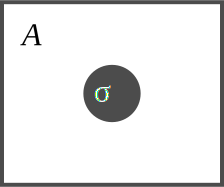
\includegraphics{sigma}
  \caption{Cross section probability}
  \label{fig:sigma}
\end{figure}
Assuming that an interaction will occur (with 100\% probability) if the projectile hits the solid, and not at all (0\% probability) if it misses, the total interaction probability for the single projectile will be
\begin{align}
  \label{eq:pssigma}
  P_S=\frac{\sigma}{A}\,.
\end{align}
Now suppose we have a parallel beam with density of particles $n$ and velocity $v$ towards the target. In time $t$, this beam fills a volume 
\begin{align}
  V=A v t\,.
\end{align}
Choosing $t$ such that the volume contains just one particle, we can write
\begin{align}
  n=1/V\,,
\end{align}
or
\begin{align}
  1=n v t A\,.
\end{align}
replacing back in \eqref{eq:pssigma} we have
\begin{align}
\sigma=\frac{P_s}{n v t}\,.  
\end{align}
$P_s$ is just the decay probability in eq.~\eqref{eq:w2}. Therefore
\begin{align}
  \sigma=\frac{\omega_2}{n v T}=&
\frac{1}{n v T}\int\ldots\int 
(2\pi)^4\delta^{(4)}\left(p_1+p_2-\sum_i k_j\right)VT 
\left|\mathcal{M}_{fi}\right|^2
\frac{1}{2E_{\mathbf{p}_1}V}\frac{1}{2E_{\mathbf{p}_2}V}
\prod_{j=1}^n\frac{d^3k_j}{(2\pi)^32E_{\mathbf{k}_j}}
\nonumber\\
=&\frac{1}{n v V}\int\ldots\int 
(2\pi)^4\delta^{(4)}\left(p_1+p_2-\sum_i k_j\right)
\left|\mathcal{M}_{fi}\right|^2
\frac{1}{2E_{\mathbf{p}_1}}\frac{1}{2E_{\mathbf{p}_2}}
\prod_{j=1}^n\frac{d^3k_j}{(2\pi)^32E_{\mathbf{k}_j}}\,.
\end{align}
The density of particles of the incident state is normalized to one particle  in the entire volume, so that $n=1/V$. Therefore
\begin{align}
   \sigma=&\frac{1}{v}\int\ldots\int 
(2\pi)^4\delta^{(4)}\left(p_1+p_2-\sum_i k_j\right)
\left|\mathcal{M}_{fi}\right|^2
\frac{1}{2E_{\mathbf{p}_1}}\frac{1}{2E_{\mathbf{p}_2}}
\prod_{j=1}^n\frac{d^3k_j}{(2\pi)^32E_{\mathbf{k}_j}}\,.
\end{align}
In general, as both particles may be moving we could use the relative velocity between them, $v_{\text{rel}}$,
\begin{align}
   \sigma=&\frac{1}{v_{\text{rel}}}\int\ldots\int 
(2\pi)^4\delta^{(4)}\left(p_1+p_2-\sum_i k_j\right)
\left|\mathcal{M}_{fi}\right|^2
\frac{1}{2E_{\mathbf{p}_1}}\frac{1}{2E_{\mathbf{p}_2}}
\prod_{j=1}^n\frac{d^3k_j}{(2\pi)^32E_{\mathbf{k}_j}}\,.
\end{align}
In a frame where $\mathbf{p}_1$ and $\mathbf{p}_2$ are along the same line, this reduces to
\begin{align}
  v_{\text{rel}}=\left|
    \frac{\mathbf{p}_1}{E_1}-\frac{\mathbf{p}_2}{E_2}
  \right|\,.
\end{align}
In fact, for not relativistic particles, where $E_i=m_i$, this coincides with the usual relative velocity
\begin{align}
   v_{\text{rel}}=&\left|
    \frac{m_1\mathbf{v}_1}{E_1}-\frac{m_2\mathbf{v}_2}{E_2}
  \right|\nonumber\\
=&\left|
    \mathbf{v}_1-\mathbf{v}_2
  \right|\,.
\end{align}
The most general formula for the relative velocity is 
\begin{align}
  v_{\text{rel}}=\frac{I}{E_1E_2}
\end{align}
where
\begin{align}
  I=&\sqrt{(p_1\cdot p_2)^2-m_1^2m_2^2}  
\end{align}

In general
\begin{align}
  I=&\sqrt{(E_1 E_2-\mathbf{p}_1\cdot\mathbf{p}_2)^2-m_1^2m_2^2}\nonumber\\
  =&\sqrt{E_1^2E_2^2+(\mathbf{p}_1\cdot\mathbf{p}_2)^2-2E_1 E_2\mathbf{p}_1.\mathbf{p}_2 -m_1^2m_2^2}
\end{align}

Since
\begin{align}
  m_1^2m_2^2=&(E_1^2-\mathbf{p}_1^2)(E_2^2-\mathbf{p}_2^2)\nonumber\\
=&(E_1^2E_2^2-\mathbf{p}_1^2E_2^2-E_1^2\mathbf{p}_2^2+\mathbf{p}_1^2\mathbf{p}_2^2)
\end{align}
\begin{align}
  I=\sqrt{\mathbf{p}_1^2E_2^2-2E_1 E_2\mathbf{p}_1\cdot\mathbf{p}_2+E_1^2\mathbf{p}_2^2
+(\mathbf{p}_1\cdot\mathbf{p}_2)^2-
\mathbf{p}_1^2\mathbf{p}_2^2}
\end{align}
If
\begin{align}
  (\mathbf{p}_1\cdot\mathbf{p}_2)^2-
\mathbf{p}_1^2\mathbf{p}_2^2=0
\end{align}
that implies that $\mathbf{p}_1$ and $\mathbf{p}_2$ are colineals,
\begin{align}
  I=&\sqrt{\mathbf{p}_1^2E_2^2-2E_1 E_2\mathbf{p}_1\cdot\mathbf{p}_2+E_1^2\mathbf{p}_2^2}
  \nonumber\\
  =&\sqrt{(\mathbf{p}_1E_2-\mathbf{p}_2E_1)^2}\nonumber\\
  =&|\mathbf{p}_1E_2-\mathbf{p}_2E_1|
\end{align}
\begin{align}
\label{eq:53}
v_{\text{rel}}=  \frac{I}{E_1E_2}=\left|
    \frac{\mathbf{p}_1}{E_1}-\frac{\mathbf{p}_2}{E_2}
  \right|
\end{align}


\begin{borrar}
Consider the collission of a cloud of particles of density $n_1^0$ moving to the right with velocity $v_1^0$ toward another cloud of particles in rest of density $n_2^0$. The differential of number of collisions is
\begin{align}
  d N\propto&|\mathbf{v}_1^0| n_1^0 n_2^0 \,d V\, dt\nonumber\\
  =&\sigma|\mathbf{v}_1^0| n_1^0 n_2^0 \,d V\, dt
\end{align}
Hence,  $\sigma$ have units of area, and corresponds to the cross section. 

The Lorentz invariant expression for velocities and particle densities is
\begin{align}
  |\mathbf{v}_1|^0 n_1^0 n_2^0\to n_1 n_2 \sqrt{(\mathbf{v}_1-\mathbf{v}_2)^2-(\mathbf{v}_1\times\mathbf{v}_2)^2}
\end{align}
Therefore
\begin{align}
  d N =&\sigma\sqrt{(\mathbf{v}_1-\mathbf{v}_2)^2-(\mathbf{v}_1\times\mathbf{v}_2)^2}n_1 n_2 \,d V\, dt  \nonumber\\
  =&\sigma\sqrt{(\mathbf{v}_1-\mathbf{v}_2)^2-(\mathbf{v}_1\times\mathbf{v}_2)^2}\frac{1}{V}(n_1V)(n_2 \,d V)\, dt\nonumber\\
 =&\sigma\sqrt{(\mathbf{v}_1-\mathbf{v}_2)^2-(\mathbf{v}_1\times\mathbf{v}_2)^2}\frac{1}{V}N_1(n_2 \,d V)\, dt\,.
\end{align}
Integrate it out
\begin{align}
  N=&\sigma\sqrt{(\mathbf{v}_1-\mathbf{v}_2)^2-(\mathbf{v}_1\times\mathbf{v}_2)^2}\frac{1}{V}N_1N_2 T
\end{align}
The probability for the collision to happens is
\begin{align}
  \label{eq:52}
  \frac{N}{N_1 N_2}=\frac{\sigma T}{V}\sqrt{(\mathbf{v}_1-\mathbf{v}_2)^2-(\mathbf{v}_1\times\mathbf{v}_2)^2}
\end{align}
The collision probability is according eq.~\eqref{eq:147}
\begin{align}
   \frac{N}{N_1 N_2}
=&\int\ldots\int 
(2\pi)^4\delta^{(4)}\left(p-\sum_i k_j\right)VT 
\left|\mathcal{M}_{fi}\right|^2
\frac{1}{2E_{\mathbf{p}_1}V}\frac{1}{2E_{\mathbf{p}_2}V}
\prod_{j=1}^n\frac{d^3k_j}{(2\pi)^32E_{\mathbf{k}_j}}
\end{align}
Replacing back in eq.~\eqref{eq:52}, we have that the  cross section is
\begin{align}
  \sigma=&\frac{V}{T\sqrt{(\mathbf{v}_1-\mathbf{v}_2)^2-(\mathbf{v}_1\times\mathbf{v}_2)^2}}\nonumber\\
&\times\int\ldots\int 
(2\pi)^4\delta^{(4)}\left(p_1+p_2-\sum_i k_j\right)VT 
\left|\mathcal{M}_{fi}\right|^2
\frac{1}{2E_{\mathbf{p}_1}V}\frac{1}{2E_{\mathbf{p}_2}V}
\prod_{j=1}^n\frac{d^3k_j}{(2\pi)^32E_{\mathbf{k}_j}}
\end{align}
Defining
\begin{align}
  I=E_{\mathbf{p}_1} E_{\mathbf{p}_2} \sqrt{(\mathbf{v}_1-\mathbf{v}_2)^2-(\mathbf{v}_1\times\mathbf{v}_2)^2}
\end{align}
we have the differential cross section as
\begin{align}
  d\sigma=&\frac{V E_{\mathbf{p}_1} E_{\mathbf{p}_2} }{T I}
(2\pi)^4\delta^{(4)}\left(p_1+p_2-\sum_i k_j\right)VT 
\left|\mathcal{M}_{fi}\right|^2
\frac{1}{2E_{\mathbf{p}_1}V}\frac{1}{2E_{\mathbf{p}_2}V}
\prod_{j=1}^n\frac{d^3k_j}{(2\pi)^32E_{\mathbf{k}_j}}
\end{align}
In this way, when the initial state in the $S$--matrix contains two particles
\begin{align}
  d\sigma=(2\pi)^4\delta^{(4)}\left(\sum_{i=1,2} p_i-\sum_{j}k_j\right)
\frac{1}{4I}\left|\mathcal{M}_{fi}\right|^2
\prod_{j}\frac{d^3k_j}{(2\pi)^32E_{\mathbf{k}_j}}
\end{align}
where
\begin{align}
  I=&\sqrt{(p_1\cdot p_2)^2-m_1^2m_2^2}\nonumber\\
=&E_{\mathbf{p}_1} E_{\mathbf{p}_2} \sqrt{(\mathbf{v}_1-\mathbf{v}_2)^2-(\mathbf{v}_1\times\mathbf{v}_2)^2}
\end{align}
Defining 
\begin{align}
  v_{\text{rel}}=\frac{I}{E_1E_2}
\end{align}
In general
\begin{align}
  I=&\sqrt{(E_1 E_2-\mathbf{p}_1\cdot\mathbf{p}_2)^2-m_1^2m_2^2}\nonumber\\
  =&\sqrt{E_1^2E_2^2+(\mathbf{p}_1\cdot\mathbf{p}_2)^2-2E_1 E_2\mathbf{p}_1.\mathbf{p}_2 -m_1^2m_2^2}
\end{align}

Since
\begin{align}
  m_1^2m_2^2=&(E_1^2-\mathbf{p}_1^2)(E_2^2-\mathbf{p}_2^2)\nonumber\\
=&(E_1^2E_2^2-\mathbf{p}_1^2E_2^2-E_1^2\mathbf{p}_2^2+\mathbf{p}_1^2\mathbf{p}_2^2)
\end{align}
\begin{align}
  I=\sqrt{\mathbf{p}_1^2E_2^2-2E_1 E_2\mathbf{p}_1\cdot\mathbf{p}_2+E_1^2\mathbf{p}_2^2
+(\mathbf{p}_1\cdot\mathbf{p}_2)^2-
\mathbf{p}_1^2\mathbf{p}_2^2}
\end{align}
If
\begin{align}
  (\mathbf{p}_1\cdot\mathbf{p}_2)^2-
\mathbf{p}_1^2\mathbf{p}_2^2=0
\end{align}
that implies that $\mathbf{p}_1$ and $\mathbf{p}_2$ are colineals,
\begin{align}
  I=&\sqrt{\mathbf{p}_1^2E_2^2-2E_1 E_2\mathbf{p}_1\cdot\mathbf{p}_2+E_1^2\mathbf{p}_2^2}
  \nonumber\\
  =&\sqrt{(\mathbf{p}_1E_2-\mathbf{p}_2E_1)^2}\nonumber\\
  =&|\mathbf{p}_1E_2-\mathbf{p}_2E_1|
\end{align}
\begin{align}
\label{eq:53}
v_{\text{rel}}=  \frac{I}{E_1E_2}=\left|
    \frac{\mathbf{p}_1}{E_1}-\frac{\mathbf{p}_2}{E_2}
  \right|
\end{align}
\end{borrar}
To simplify the notation we set $E_i=E_{\mathbf{p}_i}=$, and $E_f=E_{\mathbf{p}_f}$. Moreover, the differential cross section is
\begin{align}
    d\sigma=&(2\pi)^4\delta^{(4)}\left(\sum_{i=1}^2p_i-\sum_{f} p_f\right)
\frac{1}{4v_{\text{rel}}E_1E_2}\left|\mathcal{M}_{fi}\right|^2
\prod_{f}\frac{d^3k_f}{(2\pi)^32E_{f}}\nonumber\\
&=(2\pi)^4\frac{1}{4v_{\text{rel}}E_1E_2}\left|\mathcal{M}_{fi}\right|^2
d\Phi^{n}(p_1,p_2;k_1,\ldots,k_n)
\end{align}
where
\begin{align}
  \label{eq:50}
    d \Phi^{(n)} (p_1,p_2; k_1, k_2,\dots, k_n) = \delta^{(4)}\left(p-\sum_j k_j\right)  \prod_{j=1}^n \frac{d^3 k_j}{(2\pi)^3 2 E_{\mathbf{k}_j}} \,.
\end{align}
We keep the diferential notation both for $d\sigma$, and $d\Phi$ until the last integration have been made.

\subsection{2--to--2 cross section}
\label{sec:2-2-cross}

The the 2--to--2 cross section is
\begin{align}
 \label{eq:54}
  d\sigma=&\frac{(2\pi)^4}{4v_{\text{rel}}E_1E_2}\left|\mathcal{M}_{fi}\right|^2
d\Phi^{2}(p_1,p_2;p'_1,p'_2)\nonumber\\
=&\frac{2^4\pi^4}{2^{8}\pi^64v_{\text{rel}}E_1E_2}2^{8}\pi^6\left|\mathcal{M}_{fi}\right|^2
d\Phi^{n}(p_1,p_2;k_1,\ldots,k_n)\nonumber\\
=&\frac{1}{2^{6}\pi^2v_{\text{rel}}E_1E_2}\left|\mathcal{M}_{fi}\right|^2
\left[4(2\pi)^6d\Phi^{2}(p_1,p_2;p'_1,p'_2)\right]\nonumber\\
=&\frac{1}{64\pi^2v_{\text{rel}}E_1E_2}\left|\mathcal{M}_{fi}\right|^2
\left[4(2\pi)^6d\Phi^{2}(p_1,p_2;p'_1,p'_2)\right]
\end{align}
where, as in eq.~\eqref{eq:50}
\begin{align}
4(4\pi)^6d\Phi^{(2)}(p_1,p_2;p_1',p_2')&= \frac{4(4\pi)^6}{4(2\pi)^6} \delta^{(4)}\left(p_1+p_2-p_1'-p_2'\right)
\frac{d^3p_1'}{E_{1}'}\frac{d^3p_2'}{E_{2}'}\nonumber\\
&=  \delta^{(4)}\left(p_1+p_2-p_1'-p_2'\right)4(2\pi)^6
\frac{d^3p_1'}{E_{1}'}\frac{d^3p_2'}{E_{2}'}
\end{align}
We now will find an expression for cross section in the center of mass frame (CM) 


The center of mass (CM) frame is defined by the condition
\begin{align}
  \label{eq:55}
  \mathbf{p}_1+\mathbf{p}_2=0
\end{align}


The $\delta$--function in Eq.~\eqref{eq:101}
\begin{align}
\label{eq:56}
  \delta^{(4)}(p+p_2-p_1'-p_2')=\delta^{(3)}(\mathbf{p}_1+\mathbf{p}_2-\mathbf{p}_1'-\mathbf{p}_2')
\delta(E_1+E_2-E_1'-E_2')
\end{align}
In the CM frame
\begin{align}
\label{eq:148}
  \delta^{(4)}(p+p_2-p_1'-p_2')=\delta^{(3)}(\mathbf{p}_1'+\mathbf{p}_2')
\delta(E_1+E_2-E_1'-E_2')
\end{align}
$\mathcal{M}_{fi}$ in integration does not depend on $|\mathbf{p}_1'|$ or $|\mathbf{p}_2'|$ as the final momentum is fixed by the initial momentum whenever the final states have only two particles. In this way the integration on $p_2'$ can be evaluated directly for $d\Phi^{(2)}$. Replacing back in Eq.~\eqref{eq:54}
\begin{align}
\label{eq:149}
  4(2\pi)^6d\Phi^{(2)}=&\delta^{(3)}(\mathbf{p}_1'+\mathbf{p}_2')\delta(E_1+E_2-E_1'-E_2')
\frac{d^3p_1'}{E_{1}'}\frac{d^3p_2'}{E_{2}'}\nonumber\\
 =&\delta(E_1+E_2-E_1'-E_2')
\frac{d^3p_1'}{E_{1}'}\int\delta^{(3)}(\mathbf{p}_1'+\mathbf{p}_2')\frac{d^3p_2'}{E_{2}'}\nonumber\\
=&\delta(E_1+E_2-E_1'-E_2')
\frac{d^3p_1'}{E_{1}'E_{2}'}
\end{align}

\begin{align}
  4(2\pi)^6d\Phi^{(2)}=\delta(E_1+E_2-E_1'-E_2')
  \frac{{\mathbf{p}_1'}^2d|\mathbf{p}_1'|d\Omega}{E_{1}'E_{2}'}
\end{align}

As
\begin{align}
  |\mathbf{p}_1'|=\sqrt{{E_1'}^2-{m_1}^2}
\end{align}

\begin{align}
  \frac{d|\mathbf{p}_1'|}{dE_1'}=&\frac{2E_1'}{2\sqrt{{E_1'}^2-{m_1}^2}}\nonumber\\
  =&\frac{E_1'}{|\mathbf{p}_1'|}
\end{align}
In this way, we can write, in general
\begin{align}
 |\mathbf{p}|\, d|\mathbf{p}|=E\,dE
\end{align}
and
\begin{align}
\label{eq:57}
 4(2\pi)^6 d\Phi^{(2)}&=\delta(E_1+E_2-E_1'-E_2')
\frac{|\mathbf{p}_1'|E_1'dE_1'}{E_{1}'E_{2}'}d\Omega\nonumber\\
  &=\delta(E_1+E_2-E_1'-E_2')
\frac{|\mathbf{p}_1'|dE_1'}{E_{2}'}d\Omega
\end{align}
From the $\delta$--function in Eq.~\eqref{eq:56} we have that in the CM frame
\begin{align}
  \mathbf{p}_1+\mathbf{p}_2-\mathbf{p}_1'-\mathbf{p}_2'=0 \overset{\text{CM}}{\Rightarrow}
  \begin{cases}
    \mathbf{p}_1=-\mathbf{p}_2\\
    \mathbf{p}_1'=-\mathbf{p}_2'\\
  \end{cases}
\end{align}

Squaring the first expression, and taking into account that
\begin{align}
  \label{eq:58}
  {\mathbf{p}'_1}= \sqrt{{E_1'}^2-{m_1'}^2}
\end{align}
we have
\begin{align}
  {\mathbf{p}'_1}^2=&{\mathbf{p}'_2}^2\nonumber\\
  {E_1'}^2-{m_1'}^2=&  {E_2'}^2-{m_2'}^2\,,
\end{align}
\begin{align}
\label{eq:59}
  E_2'=\sqrt{{E_1'}^2-{m_1'}^2+{m_2'}^2}
\end{align}
In this way we can express $E_2'$ in terms of $E_1'$ in Eq.~\eqref{eq:57}.
Moreover, we can define the center of mass energy as
\begin{align}
  \label{eq:60}
  \sqrt{s}=E_1+E_2
\end{align}
Using The energy part of $\delta$--function in Eq.~\eqref{eq:56} can be written as
\begin{align}
  \delta\left(\sqrt{s}-E_1'-\sqrt{{E_1'}^2-{m_1'}^2+{m_2'}^2}\right)
\end{align}
As established before,  $\mathcal{M}_{fi}$ in this case in independent of $|\mathbf{p}'_1|$, and the integration on $E_1'$ can be done directly only for $d\Phi^{(2)}$.
The integral is easily performed using the identity
\begin{align}
  \delta\left(f(z)\right)=\sum_n\frac{\delta(z-z_n)}{|f'(z_n)|}
\end{align}
where $z_n$ are the zeroes of $f(z)$. In this case, this $\delta$--function is a function of the integration variable $E_1'$, with only one zero
\begin{align}
   \delta\left(f(x)\right)=\frac{\delta(x-x_0)}{|f'(x_0)|}
\end{align}
where
\begin{align}
  f(x)=\sqrt{s}-x-\sqrt{x^2-{m_1'}^2+{m_2'}^2}
\end{align}
Therefore
\begin{align}
  \label{eq:61}
   4(2\pi)^6d\Phi^{(2)}=&d\Omega\int\frac{\delta(x-x_0)}{|f'(x_0)|}\frac{
     |\mathbf{p}_1'(x)|}{E_2'(x)}dx\nonumber\\
   =&d\Omega\frac{1}{|f'(x_0)|}\frac{
     |\mathbf{p}_1'(x_0)|}{E_2'(x_0)}\nonumber\\
\end{align}
where from Eqs.~\eqref{eq:58}, \eqref{eq:59},
\begin{align}
  \label{eq:62}
  \mathbf{p}_1'(x_0)=&\sqrt{x_0^2-{m_1'}^2}&
  E_2'(x_0)=&\sqrt{x_0^2-{m_1'}^2+{m_2'}^2}
\end{align}
The zero is obtained from
\begin{align}
  &\sqrt{s}-x_0-\sqrt{x_0^2-{m_1'}^2+{m_2'}^2}=0\nonumber\\
  &s-2\sqrt{s}\,x_0+x_0^2=x_0^2-{m_1'}^2+{m_2'}^2\nonumber\\
  &s-2\sqrt{s}\,x_0=-{m_1'}^2+{m_2'}^2
\end{align}
with solution
\begin{align}
  \label{eq:63}
  x_0=\frac{s+{m_1'}^2-{m_2'}^2}{2\sqrt{s}}
\end{align}
As (See 
\texttt{deltaxn.nb} %noinstiki [deltax.nb](Appendix)
for additional details)
\begin{align}
  f'(x)=-\frac{x}{\sqrt{x^2-{m_1'}^2+{m_2'}^2}}-1
\end{align}
we have
\begin{align}
  \label{eq:64}
  f'(x_0)=&-\frac{{m_1'}^2-{m_2'}^2+s}{\sqrt{s}
   \sqrt{\frac{\left(-{m_1'}^2+{m_2'}^2+s\right)^2}{s}}}-1\nonumber\\
    =&\frac{-{m_1'}^2+{m_2'}^2-s}{-{m_1'}^2+{m_2'}^2+s}-1\nonumber\\
    =&\frac{-{m_1'}^2+{m_2'}^2-s+{m_1'}^2-{m_2'}^2-s}{-{m_1'}^2+{m_2'}^2+s}\nonumber\\
=&\frac{-2s}{s+{m_2'}^2-{m_1'}^2}\,,
\end{align}
and
\begin{align}
  \label{eq:65}
  \delta(f(E_1'))=\delta(E_1'-x_0)\left(\frac{s+{m_2'}^2-{m_1'}^2}{2s}\right)
\end{align}

Replacing the expression for $x_0$ in \eqref{eq:63} into Eq.~\eqref{eq:62} we have (See 
\texttt{deltaxn.nb}  %noinstiki [deltax.nb](Appendix)
for additional details)
\begin{align}
  \label{eq:66}
   \mathbf{p}_1'(x_0)=&\frac{\sqrt{[s-({m_1'}-{m_2'})^2][s-({m_1'}+{m_2'})^2]}}{2\sqrt{s}}\nonumber\\
E_2'(x_0)=&  \frac{s-{m_1'}^2+{m_2'}^2}{2\sqrt{s}}
\end{align}

Replacing Eqs.~\eqref{eq:64}, and \eqref{eq:66} in Eq.~\eqref{eq:61}
we have
\begin{align}
  \label{eq:67}
4(2\pi)^6d\Phi^{(2)}&=d\Omega\frac{1}{|f'(x_0)|}
\frac{\sqrt{x_0^2-{m_1'}^2}}{\sqrt{x_0^2-{m_1'}^2+{m_2'}^2}}\nonumber\\
  &=d\Omega\left(\frac{s-{m_1'}^2+{m_2'}^2}{2s}\right)
\frac{\sqrt{[s-({m_1'}-{m_2'})^2][s-({m_1'}+{m_2'})^2]}}{s-{m_1'}^2+{m_2'}^2}\nonumber\\
&=d\Omega\frac{\sqrt{[s-({m_1'}-{m_2'})^2][s-({m_1'}+{m_2'})^2]}}{2s}
\end{align}
Defining the kinematic two particle function
\begin{align}
  \label{eq:46}
  \lambda(a,b,c)\equiv(a-b+c)^2-4ac
\end{align}
and taking into account that
\begin{align}
  \left(s-{m_2'}^2+{m_1'}^2\right)^2-4s{m_1'}^2=[s-({m_1'}-{m_2'})^2][s-({m_1'}+{m_2'})^2]
\end{align}
we have
\begin{align}
\label{eq:150}
  4(2\pi)^6d\Phi^{(2)}=d\Omega\frac{\lambda^{1/2}(s,{m_2'}^2,{m_1'}^2)}{2s}
\end{align}
Moreover
\begin{align}
  \label{eq:151}
  \mathbf{p}_1'=&\frac{\lambda^{1/2}(s,{m_2'}^2,{m_1'}^2)}{2\sqrt{s}}
\end{align}
%\left(\right)

To further evaluate Eq.~(\ref{eq:54}), we need to express $v_{\text{rel}}$ and $E_1E_2$ in terms of $s$ and the masses. Concerning $v_{\text{rel}}$,
from Eq.~\eqref{eq:53}, evaluated in CM frame
\begin{align}
  \label{eq:68}
    E_1E_2 v_{\text{rel}}=&E_1E_2\left|\frac{\mathbf{p}_1}{E_1}-\frac{\mathbf{p}_2}{E_2}\right|\nonumber\\
  =&E_1E_2\left|\frac{\mathbf{p}_1}{E_1}+\frac{\mathbf{p}_1}{E_2}\right|\nonumber\\
  =&\left|\mathbf{p}_1\right|({E_1+E_2})\nonumber\\
  =&\left|\mathbf{p}_1\right|\sqrt{s}
\end{align}
Replacing back Eqs.~\eqref{eq:67}, and \eqref{eq:68} into Eq.~\eqref{eq:54}, we have
\begin{align}
  \label{eq:69}
      d\sigma=&\frac{1}{64\pi^2E_1E_2v_{\text{rel}}}\overline{\left|\mathcal{M}_{fi}\right|^2}
    \left[4(2\pi)^6d\Phi^{(2)}\right]
\end{align}
\begin{align}
  \frac{d\sigma}{d\Omega}=\frac{1}{64\pi^2E_1E_2v_{\text{rel}}}\overline{\left|\mathcal{M}_{fi}\right|^2}
\frac{\sqrt{[s-({m_1'}+{m_2'})^2][s-({m_1'}-{m_2'})^2]}}{2s}
\end{align}
By using Eq.~\eqref{eq:68}
\begin{align}
  \frac{d\sigma}{d\Omega}=\frac{1}{64\pi^2|\mathbf{p}_1|\sqrt{s}}\overline{\left|\mathcal{M}_{fi}\right|^2}
\frac{\sqrt{[s-({m_1'}+{m_2'})][s-({m_1'}^2-{m_2'}^2)]}}{2s}
\end{align}
In the CM frame
\begin{align}
\sqrt{s}=&E_1+E_2\nonumber\\
=&\sqrt{\mathbf{p}_1^2+m_1^2}+\sqrt{\mathbf{p}_2^2+m_2^2}\nonumber\\
=&\sqrt{\mathbf{p}_1^2+m_1^2}+\sqrt{\mathbf{p}_1^2+m_2^2}
\end{align}

\begin{align}
  \label{eq:70}
  s=&2\mathbf{p}_1^2+m_1^2+m_2^2+2\sqrt{\mathbf{p}_1^4+(m_1^2+m_2^2)\mathbf{p}_1^2+m_1^2m_2^2}\nonumber\\
s-(2\mathbf{p}_1^2+m_1^2+m_2^2)=&2\sqrt{\mathbf{p}_1^4+(m_1^2+m_2^2)\mathbf{p}_1^2+m_1^2m_2^2}
\end{align}
\begin{align}
  s^2-2s(2\mathbf{p}_1^2+m_1^2+m_2^2)+[2\mathbf{p}_1^2+(m_1^2+m_2^2)]^2=&4(\mathbf{p}_1^4+(m_1^2+m_2^2)\mathbf{p}_1^2+m_1^2m_2^2)\nonumber\\
  s^2-2s(2\mathbf{p}_1^2+m_1^2+m_2^2)+4\mathbf{p}_1^4+4\mathbf{p}_1^2(m_1^2+m_2^2)
+(m_1^2+m_2^2)^2=&4(\mathbf{p}_1^4+(m_1^2+m_2^2)\mathbf{p}_1^2+m_1^2m_2^2)\nonumber\\
-4s\mathbf{p}_1^2+s^2-2s(m_1^2+m_2^2)+(m_1^2+m_2^2)^2=&4m_1^2m_2^2\nonumber\\
-4s\mathbf{p}_1^2+s^2-2sm_1^2-2sm_2^2+m_1^4+m_2^4+2m_1^2m_2^2=&4m_1^2m_2^2\nonumber\\
-4s\mathbf{p}_1^2+s^2-2sm_1^2-2sm_2^2+m_1^4+m_2^4-2m_1^2m_2^2=&0
\end{align}
\begin{align}
  \mathbf{p}_1^2=\frac{\left(s-m_1^2-2 m_2 m_1-m_2^2\right)
   \left(s-m_1^2+2 m_2m_1-m_2^2\right)}
{4s}
\end{align}
\begin{align}
  \label{eq:71}
  |\mathbf{p}_1|=&\frac{\sqrt{[s-(m_1+m_2)^2][s-(m_1-m_2)^2]}}{2\sqrt{s}}\nonumber\\
=&\frac{\lambda^{1/2}(s,m_2^2,m_1^2)}{2\sqrt{s}}
\end{align}
Replacing Eq.~\eqref{eq:71} back in Eq.~\eqref{eq:68} we have
\begin{align}
  \label{eq:72}
  E_1E_2 v_{\text{rel}}=\frac{1}{2}\sqrt{[s-(m_1+m_2)^2][s-(m_1-m_2)^2]}
\end{align}
Replacing Eqs.~\eqref{eq:72}, and \eqref{eq:67} in Eq.~\eqref{eq:54}
\begin{align}
  \label{eq:73}
  d\sigma=&\frac{1}{64\pi^2}\overline{\left|\mathcal{M}_{fi}\right|^2}\frac{d\Omega}{2s}(2)
\sqrt{\frac{[s-(m_1'+m_2')^2][s-(m_1'-m_2')^2]}{[s-(m_1+m_2)^2][s-(m_1-m_2)^2]}}
\end{align}
and, finally
\begin{align}
  \label{eq:74}
  \frac{d\sigma}{d\Omega}=\frac{1}{64\pi^2s}\left\{
\frac{[s-(m_1'+m_2')^2][s-(m_1'-m_2')^2]}{[s-(m_1+m_2)^2][s-(m_1-m_2)^2]}\right\}^{1/2}
\overline{|\mathcal{M}|^2}
\end{align}
or, in terms of the kinematic function defined in eq.~\eqref{eq:46}
\begin{align}
  \label{eq:74}
  \frac{d\sigma}{d\Omega}=\frac{1}{64\pi^2s}
\frac{\lambda^{1/2}(s,{m_2'}^2,{m_1'}^2)}{\lambda^{1/2}(s,m_2^2,m_1^2)}
\overline{|\mathcal{M}|^2}
\end{align}
%\left(\right)

\section{Decay Rates}
\label{sec:decay-rates}
Consider the matrix element of $i T$ in (\ref{eq:41})
\begin{align}
  \label{eq:45}
  \langle\mathbf{p}|i T|\mathbf{k}_1\ldots\mathbf{k}_n\rangle^{\text{NR}}=(2\pi)^4\delta^{(4)}\left(p-\sum_i k_i\right)i{M}_{fi}
\end{align}

where the initial state is a single particle of momentum $p$ and mass $M$, while the final state is given by $n$ particles of momenta $k_i$ and masses $m_i$, $i=1,\ldots,n$. 
We are therefore considering a decay process. 


By using eq.~\eqref{eq:146} we have
\begin{align}
\omega=&\int\ldots\int 
(2\pi)^4\delta^{(4)}\left(p-\sum_i k_j\right)\left(\int dt\right) 
\left|\mathcal{M}_{fi}\right|^2
\frac{1}{2E_{\mathbf{p}}}
\prod_{j=1}^n\frac{d^3k_j}{(2\pi)^32E_{\mathbf{k}_j}}
\end{align}
Therefore the differential probability is
\begin{align}
  d\omega=&\int\ldots\int 
(2\pi)^4\delta^{(4)}\left(p-\sum_i k_j\right)
\frac{1}{2E_{\mathbf{p}}}\left|\mathcal{M}_{fi}\right|^2
dt\prod_{j=1}^n\frac{d^3k_j}{(2\pi)^32E_{\mathbf{k}_j}}
\end{align}
Finally we define the \textit{decay rate} $d\Gamma$ as the decay probability in which in the final state
the j--th particle has momentum between $k_j$ and $k_j+ dk_j$ per unit time
\begin{align}
\label{eq:49}
d\Gamma\equiv&\frac{d\omega}{dt}=
(2\pi)^4\delta^{(4)}\left(p-\sum_j k_j\right)
\frac{1}{2E_{\mathbf{p}}}\left|\mathcal{M}_{fi}\right|^2
\prod_{j=1}^n\frac{d^3k_j}{(2\pi)^32E_{\mathbf{k}_j}}\nonumber\\
=&\frac{(2\pi)^4}{2E_{\mathbf{p}}}\left|\mathcal{M}_{fi}\right|^2
d \Phi^{(n)} (p; k_1, k_2,\dots, k_n)
\end{align}
where
\begin{align}
  \label{eq:50}
    d \Phi^{(n)} (p; k_1, k_2,\dots, k_n) = \delta^{(4)}\left(p-\sum_j k_j\right)  \prod_{j=1}^n \frac{d^3 k_j}{(2\pi)^3 2 E_{\mathbf{k}_j}} \,.
\end{align}
and the differential decay width in the center of mass frame
\begin{align}
  \label{eq:51}
  d\Gamma=\frac{(2\pi)^4}{2E_{\mathbf{p}}}\left|\mathcal{M}_{fi}\right|^2
d \Phi^{(n)} (p; k_1, k_2,\dots, k_n)
\end{align}

\subsection{Two body decays}
We now consider the decay of particle of mass $M$ decaying into two particles of 4--momenta $p_1$, $p_2$ and masses $m_1$, $m_2$. In the CM frame the initial momentum satisfy
\begin{align}
  \mathbf{p}=&0\Rightarrow M=E_{\mathbf{p}}
\end{align}
Therefore 
\begin{align}
  \label{eq:51}
  d\Gamma=&\frac{(2\pi)^4}{2M[4(2\pi)^6]}\left|\mathcal{M}_{fi}\right|^2
4(2\pi)^6d \Phi^{(2)} (p; p_1, p_2)\nonumber\\
=&\frac{1}{2^3M(2\pi)^2}\left|\mathcal{M}_{fi}\right|^2
4(2\pi)^6d \Phi^{(2)} (p; p_1, p_2)\nonumber\\
=&\frac{1}{32 \pi^2M}\left|\mathcal{M}_{fi}\right|^2
\left[4(2\pi)^6d \Phi^{(2)} (p; p_1, p_2)\right]
\end{align}
where
\begin{align}
  4(2\pi)^6d \Phi^{(2)} (p; p_1, p_2)=\delta^{(4)}(p-p_1-p_2)\frac{d^3p_1}{E_{1}}\frac{d^3p_2}{E_{2}}
\end{align}
The Dirac delta in eq.~\eqref{eq:50} can be written in the CM frame as
\begin{align}
\label{eq:153}
  \delta^{(4)}(p-p_1-p_2)=&\delta^{(3)}(\mathbf{p}-\mathbf{p}_1-\mathbf{p}_2)\delta(E-E_1-E_2)\nonumber\\
=&\delta^{(3)}(\mathbf{p}_1+\mathbf{p}_2)\delta(M-E_1-E_2)
\end{align}
and,
\begin{align}
   4(2\pi)^6d \Phi^{(2)} (p; p_1, p_2)=&\delta(M-E_1-E_2)\delta^{(3)}(\mathbf{p}_1+\mathbf{p}_2)\frac{d^3p_1}{E_{1}}\frac{d^3p_2}{E_{2}}
\end{align}
Comparing with eq.~\eqref{eq:149} we see that the two quantities are the same after the replacing $\sqrt{s}\to M$, $p_1'\to p_1$ and $p_2'\to p_2$. Therefore we have from eq.~\eqref{eq:150}
\begin{align}
    4(2\pi)^6d\Phi^{(2)}=d\Omega\frac{\lambda^{1/2}(M^2,m_2^2,m_1^2)}{2M^2}
\end{align}
Replacing back in eq.~\eqref{eq:51}
\begin{align}
\label{eq:152}
\frac{d\Gamma}{d\Omega}=&\frac{1}{32 \pi^2M}\left|\mathcal{M}_{fi}\right|^2\frac{\lambda^{1/2}(M^2,m_2^2,m_1^2)}{2M^2}\nonumber\\
=&\frac{1}{64 \pi^2M^3}\left|\mathcal{M}_{fi}\right|^2\lambda^{1/2}(M^2,m_2^2,m_1^2) 
\end{align}
By using eq.~\eqref{eq:151} we can write this expression also as
\begin{align}
\frac{d\Gamma}{d\Omega}
=&\frac{1}{64 \pi^2M^3}\left|\mathcal{M}_{fi}\right|^22M|\mathbf{p}_1|\nonumber\\
=&\frac{|\mathbf{p}_1|}{32 \pi^2M^2}\left|\mathcal{M}_{fi}\right|^2
\end{align}
as usually written in several texts.



\section{Backup}
\label{sec:backup}

Perturbation theory is developed more easily using the Hamiltonian formalism. We therefore consider a general field theory with a Hamiltonian
\begin{align}
  \label{eq:75}
  H=H_0+H_{\text{int}}\,
\end{align}
where $H_0$ is the free Hamiltonian and $H_{\text{int}}$ is the interaction term. The interaction term will be considered small. For instance in QED
\begin{align}
  H_{\text{int}}=\int d^3x\,\mathcal{H}_{\text{int}}=-\int d^3x\,\mathcal{L}_{\text{int}}
\end{align}
with
\begin{align}
  \mathcal{L}_{\text{int}}=-e A_\mu\overline{\psi}\gamma^\mu\psi
\end{align}
The smallnes of the interaction follows from the fact that the parameter which turns out to be relevatn for the perturbation expansion is $\alpha=e^2/4\pi\approx1/137$.


\begin{align}
  S S^\dagger=&(1+i T)(1-i T^\dagger)\nonumber\\
  &=1+i(T-T^\dagger)+T T^\dagger=1\,,\nonumber\\
\end{align}
\begin{align}
  T T^\dagger=-i(T-T^\dagger)\,.
\end{align}
Inserting a complete set of states we have
\begin{align}
  \langle b|T T^\dagger|a\rangle=&-i(\langle b|T|a\rangle-\langle b|T^\dagger|a\rangle)\nonumber\\
\langle b|T\left(\sum_n|n\rangle\langle n|\right)T^\dagger|a\rangle=&-i\left[\langle b|T|a\rangle-\left(\langle a|T|b\rangle\right)^\dagger\right]\nonumber\\
\sum_n\langle b|T|n\rangle\langle a|T|n\rangle^\dagger=&-i\left(\langle b|T|a\rangle-\langle a|T|b\rangle^*\right)\nonumber\\
\sum_n T_{bn}T_{an}^*=&-i\left(T_{ba}-T_{ab}^*\right)\,.\nonumber\\
\end{align}
if $a=b$
\begin{align}
  |T_{an}|^2=-i\operatorname{Im}T_{aa} \,.
\end{align}

%\left(\right)
%%% Local Variables: 
%%% mode: latex
%%% TeX-master: "beyond"
%%% End: